%=========================================================================================
\chapter{自适应分布式化框架}



本章节介绍本文提出的自适应分布式化框架,如图\ref{fig:overview}所示。本章首先在\ref{sec:serverless}中介绍本文对于系统的抽象模型。然后在\ref{sec:nanofunction}和\ref{sec:dismod}中介绍原子函数和分布式模块的详细内容,他们是编译器的底层原理。编译器首先在程序中识别出所有的原子函数,然后分析出原子函数之间的依赖关系,构造出原子函数调用DAG。过程中统计每个原子函数的相关指标信息。然后通过分组聚类算法将DAG中的原子函数分组构成分布式模块。以分布式模块作为最小的部署单元。通过编译器将单机程序编译成分布式模块。然后通过服务器将分布式模块部署到服务器上。最后通过执行器将分布式模块执行。后续章节分别介绍编译器、服务器和执行器的详细内容。

\begin{figure}[ht]
	\centering
    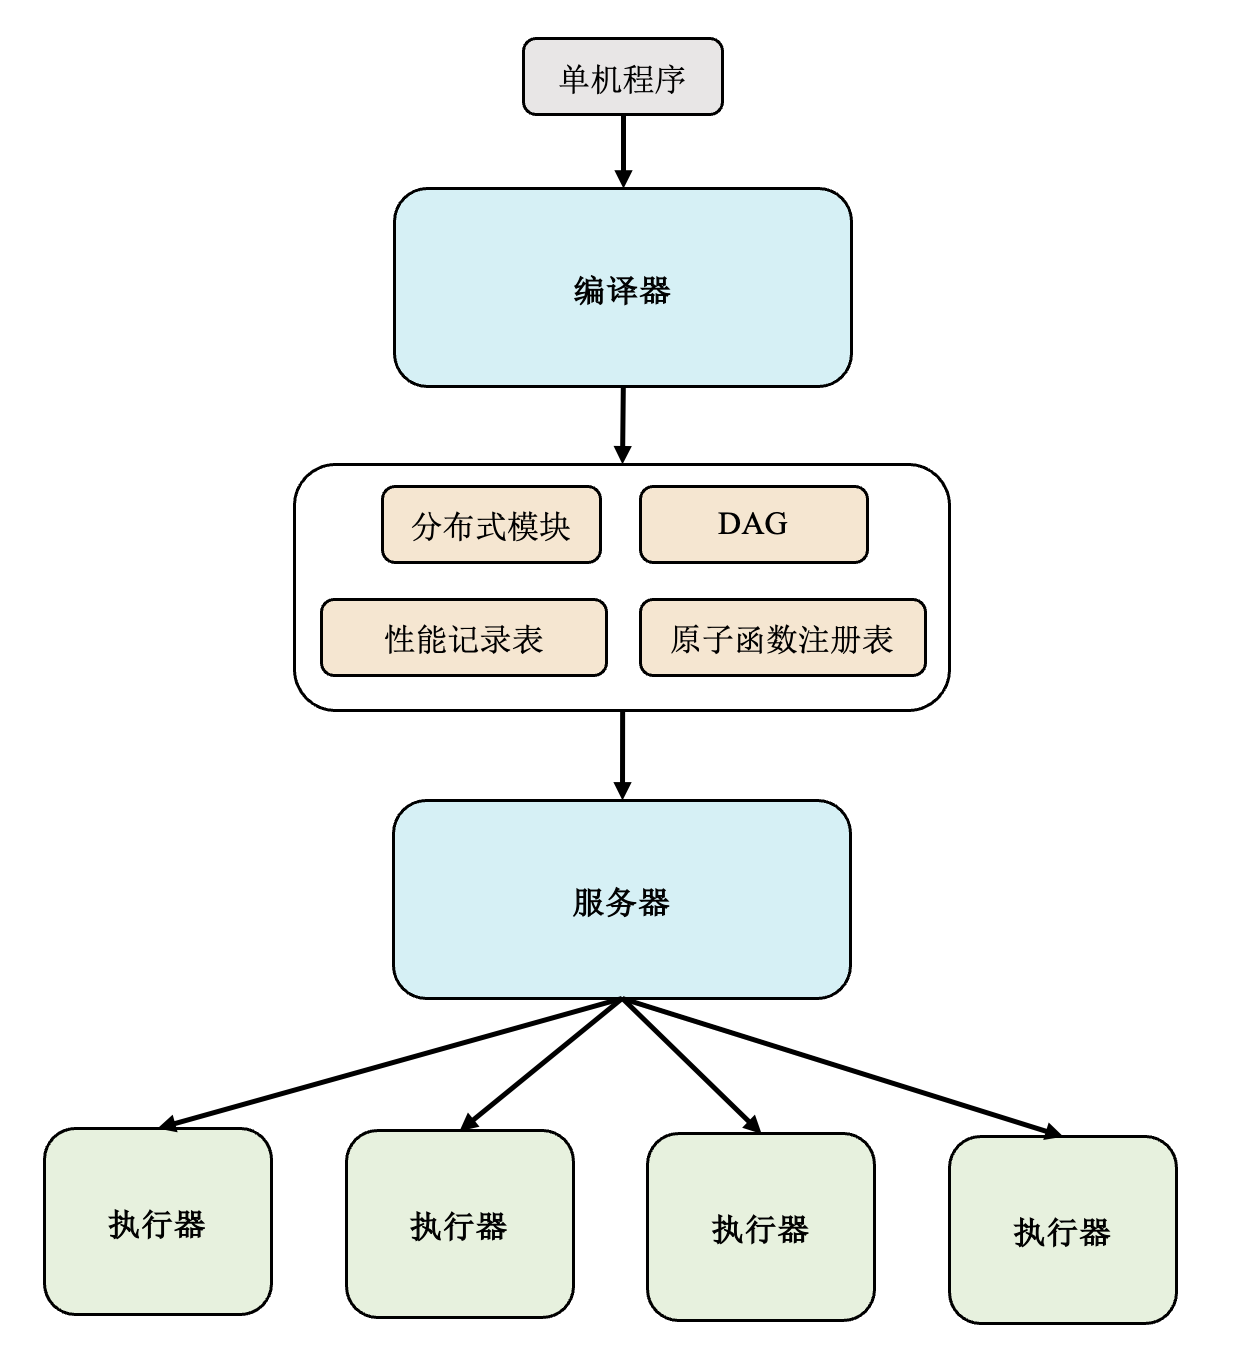
\includegraphics[width=0.6\linewidth]{das_arc.png}
    \vspace{8pt}
	\caption{自适应分布式框架的整体架构}
    \label{fig:overview}
\end{figure}

% %=========================================================================================


\section{针对程序的Serverless抽象}
\label{sec:serverless}
本文首先参考Serverless模型的抽象层次来拆分程序,将单机程序拆分为多个独立的函数单元,便于分布式部署和执行。Serverless模型具有函数粒度、无状态性、按需执行、自动扩缩容等特性。

在本文的框架中,首先识别出程序的所有函数,这些函数是最小粒度的函数单元。
函数调用在程序结构中呈现嵌套层次关系,如代码\ref{code:function_depth}所示,以一个典型Python程序为例,main函数调用foo函数,foo函数调用bar函数,bar函数继而调用Python标准库中的print函数。若考虑更细粒度的函数拆分,则理论上需要对Python标准库中的函数进行进一步分析。然而,对标准库函数进行深度拆分以分析其内部依赖关系、CPU时间消耗及内存占用特征,将显著增加框架的计算开销。此外,鉴于Python标准库中函数调用链路的复杂性,若对每个函数单元都实施分布式化处理,函数间远程调用的通信开销将呈指数级增长。

在分布式系统中,函数调用可以分为本地调用和远程调用两种形式。本地调用的开销主要包括栈帧分配、参数传递和返回值处理,通常在微秒级别;而远程调用则涉及序列化/反序列化、网络传输和协议处理等额外开销,往往达到毫秒级别,比本地调用高出2-3个数量级。因此,在确定函数拆分深度$h$时,因为在内存等限制条件下函数可能被分组到其他分布式模块中,所以需要权衡计算并行带来的性能提升与远程调用引入的通信延迟。



\begin{lstlisting}[
	language=Python,
	caption={函数嵌套调用示例},
	label={code:function_depth},
	breaklines=true,
	showstringspaces=false
]
def main():
    print("Hello, World!")
    # 调用其他函数
    result = foo(5)
    print(f"结果: {result}")
def foo(x):
    # foo函数调用bar函数
    return bar(x) * 2
def bar(x):
    # bar函数调用Python标准库函数
    print(f"在bar中处理: {x}")
    return x + 1
if __name__ == "__main__":
    main()
\end{lstlisting}

考虑到函数的嵌套深度,本文选择一个合理的函数深度$h$,来平衡函数调用的开销和函数拆分的开销。在选择的函数深度$h$上,函数单元被识别为若干个原子函数。

在原子函数的基础之上,框架通过分析原子函数之间的依赖关系,来构建原子函数调用DAG,过程中统计每个原子函数的相关指标信息。依据DAG和统计的指标信息,通过分组聚类算法将DAG中的原子函数分组构成分布式模块。以分布式模块作为最小的部署单元。

在Serverless的环境下,单机程序在本文的框架下,被编译成多个分布式模块,然后通过服务器将分布式模块部署到服务器上,最后通过执行器将分布式模块执行。


\section{原子函数}
\label{sec:nanofunction}
程序在设定的函数深度$h$上,被拆分成若干个独立的原子函数$f_{i}^{h}$,如图\ref{fig:nanofunction_dag}所示。每个原子函数分别统计CPU时间消耗、内存占用、函数依赖等信息。框架通过对原子函数$f_{i}^{h}$的CPU时间消耗和内存占用进行精确量化,构建资源消耗模型,这使构造分布式模块的分组聚类算法能够根据不同原子函数的特性进行最优化分布式模块分配。这种基于资源感知的调度策略在分布式计算理论中被证明可以显著降低总体执行时间,符合Amdahl定律和Gustafson定律所描述的并行系统性能边界。

\begin{figure}[h]
\centering
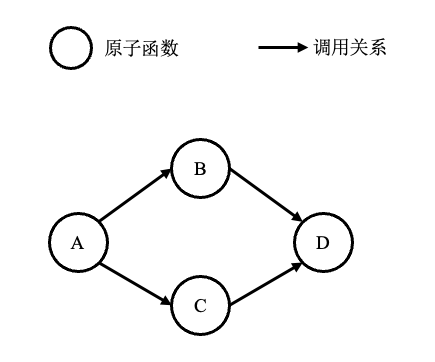
\includegraphics[width=0.4\linewidth]{nanofunction_dag.png}
\caption{原子函数调用DAG}
\label{fig:nanofunction_dag}
\end{figure}

为精确构建原子函数的调用依赖关系图,本框架采用基于抽象语法树(AST)的静态程序分析方法。在依赖图构建过程中,本文假设函数调用关系不存在环状结构,这是因为环状依赖会导致模块间的紧耦合,显著增加分布式系统中的通信开销,同时使得系统难以实现弹性扩缩容和故障隔离。当原子函数间存在复杂的循环依赖时,它们必须被部署在同一分布式模块中,这违背了本文追求的高并行度和负载均衡目标。算法描述如算法\ref{atomic_function_dag}所示。具体实现如下:

首先,将源码转换为AST表示。在AST上,框架实现了一种多阶段的算法:第一阶段识别所有原子函数定义,建立原子函数符号表$S_f^h$;第二阶段针对每个函数体$f_i^h$进行深度优先遍历,检测所有函数调用表达式节点,记录调用关系$(f_i^h, f_j^h)$到有向图$G$中。

为统计函数调用频率,框架在静态分析的基础上引入了基于控制流权重的频率估计模型。该模型从AST构建控制流图(CFG),并根据以下规则分配调用频率权重:

(1)直接函数调用赋予基础权重$w_0=1.0$。 

(2)子函数调用赋予父函数在调用处的权重$w_0$。 

(3)循环体中的调用,根据循环嵌套深度$d$,权重为$w_l=10^d$。

(4)条件分支中的调用,根据分支复杂度和位置,权重为$w_c=0.5$。

在完成函数调用频率权重的统计后,框架进一步构建原子函数调用图$G=(V, E)$,其中$V$表示所有原子函数的集合,$E$表示函数调用关系的集合。对于每一条边$(f_i^h, f_j^h) \in E$,本文赋予其权重$w(f_i^h, f_j^h)$,表示$f_i^h$调用$f_j^h$的频率。这样,本文就得到了一个加权有向无环图。

\begin{algorithm}[ht]
	\caption{原子函数识别与调用DAG构建}
	\label{atomic_function_dag}
	\SetAlgoLined
	\KwIn{源程序($P$)}
	\KwOut{原子函数集合($F$), 原子函数调用DAG($G$)}
	
	$F \gets \emptyset$; $G=(V,E) \gets (\emptyset, \emptyset)$\;
	通过静态分析提取程序$P$中的所有函数集合 $F_{all}$\;
	\ForEach{$f_i \in F_{all}$}{
		\If{$f_i\text{的函数深度}\leq h$}{
			$F \gets F \cup \{f_i\}$\;
			$V \gets V \cup \{f_i\}$\;
			\ForEach{$f_j \in f_i\text{的子函数}$}{
				$w(f_i, f_j) \gets\text{计算调用频率权重}$ \;
				$E \gets E \cup \{(f_i, f_j, w(f_i, f_j))\}$\;
			}
		}
	}
	\ForEach{$f \in F$}{
		测量$f$的CPU时间消耗和内存占用\;
		更新$f$在$V$中的属性\;
	}
	\Return{$F, G$}\;
\end{algorithm}

为获取原子函数$f_{i}^{h}$的精确性能特征,本文设计并实现了一种多维度资源监测框架。该框架基于动态程序分析理论,通过非侵入式轻量级插桩技术在原子函数的入口与出口处自动注入性能探针代码。执行时间采集利用高精度计时器实现纳秒级精度测量。内存占用监测采用了增量式页表扫描算法,结合操作系统的内存管理子系统接口,实现了$O(\Delta m)$复杂度的内存变化追踪,其中$\Delta m$为函数执行期间内存状态的变化量。为降低监测引入的性能干扰,框架实现了基于统计学原理的分层采样机制:对执行频率超过阈值$\tau$的热点函数采用$1/1$比例的全采样策略;对中等频率函数采用$1/k$的固定间隔采样;对执行频率低于阈值$\tau$的冷点函数实施自适应指数退避采样策略,使总体监测开销控制在可接受范围内。

最终构造的函数调用DAG包含了三个关键信息。节点信息记录原子函数$f_i^h$的CPU时间消耗、内存占用等资源使用情况,如表\ref{tab:consumption}所示。边信息记录函数调用关系及其频率权重。拓扑信息记录函数间的依赖层次和调用路径。

\begin{table}[ht]
		\renewcommand{\arraystretch}{0.75}
		\caption{原子函数指标统计表示例}  
        \label{tab:pointrank}
		\begin{tabularx}{\textwidth}{*{4}{>{\centering\wuhao\arraybackslash}X}}
		\toprule[1.5pt]
		函数名 & 频率 & CPU时间消耗 & 内存占用 \\ 
        \midrule[1pt]
		A  & 1.0 & 100 & 1.0\\ 
		B  & 2.0 & 200 & 2.0\\ 
		C  & 3.0 & 200 & 2.0\\
		D  & 4.0 & 30  & 3.0\\
		\bottomrule[1.5pt]
		\end{tabularx}
		\label{tab:consumption}
\end{table}

函数调用DAG提供了程序结构的整体视图,不仅反映了函数间的调用关系,还量化了这些关系的强度和资源需求。这为后续的分布式模块划分提供了数据基础,使得框架能够基于函数的资源消耗特征和调用关系进行最优化的模块分配。


\section{分布式模块}
\label{sec:dismod}
在获取原子函数调用DAG后,本文提出了一种基于资源消耗特征和通信开销的分组聚类算法来构造分布式模块。该算法旨在实现计算负载均衡与模块间通信最小化的双重优化目标。分布式模块的构造需要解决两个关键问题:一是如何将原子函数合理分组以实现负载均衡;二是如何最小化模块间的通信开销。这两个目标往往相互制约,因为追求完美的负载均衡可能导致频繁通信的函数被分配到不同模块,而过度强调通信局部性则可能造成计算资源分配不均。本文提出的算法通过权衡这两方面因素,实现了分布式模块构造算法分为三个阶段:初始化、迭代优化和通信优化。

注意到原子函数的远程调用花费时间远大于本地调用所花费的时间,因为远程调用涉及网络传输、序列化/反序列化、协议处理等额外开销,而本地调用仅需处理栈帧分配和参数传递,两者在性能上通常相差2-3个数量级。如图\ref{fig:dismod:a}将更多的依赖函数分配到同一模块以减少远程调用的开销,而图\ref{fig:dismod:b}则展示了更多远程调用发生的分组情况。所以算法需要综合地考虑到这个情况。

\begin{figure}[ht]
\centering
\subfigure[将多个依赖原子函数分组到不同分布式模块]{
    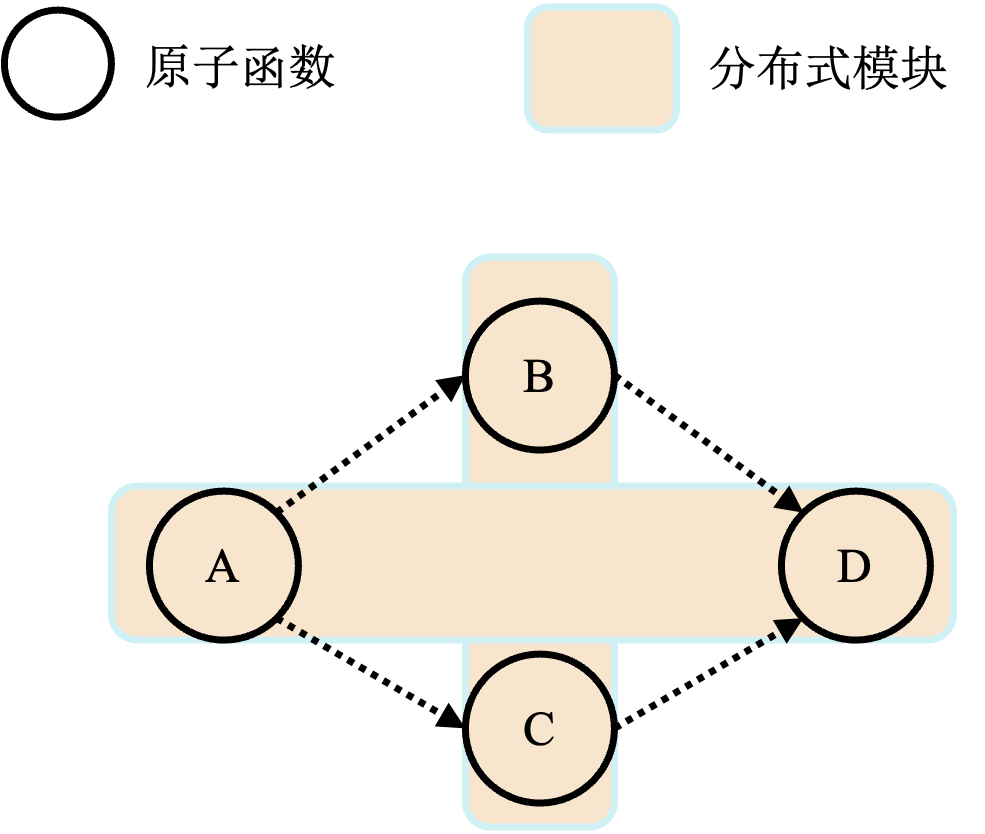
\includegraphics[width=0.48\linewidth]{figures/remote.png}
    \label{fig:dismod:a}
}
\hfill
\subfigure[将多个依赖原子函数分组到同一分布式模块]{
    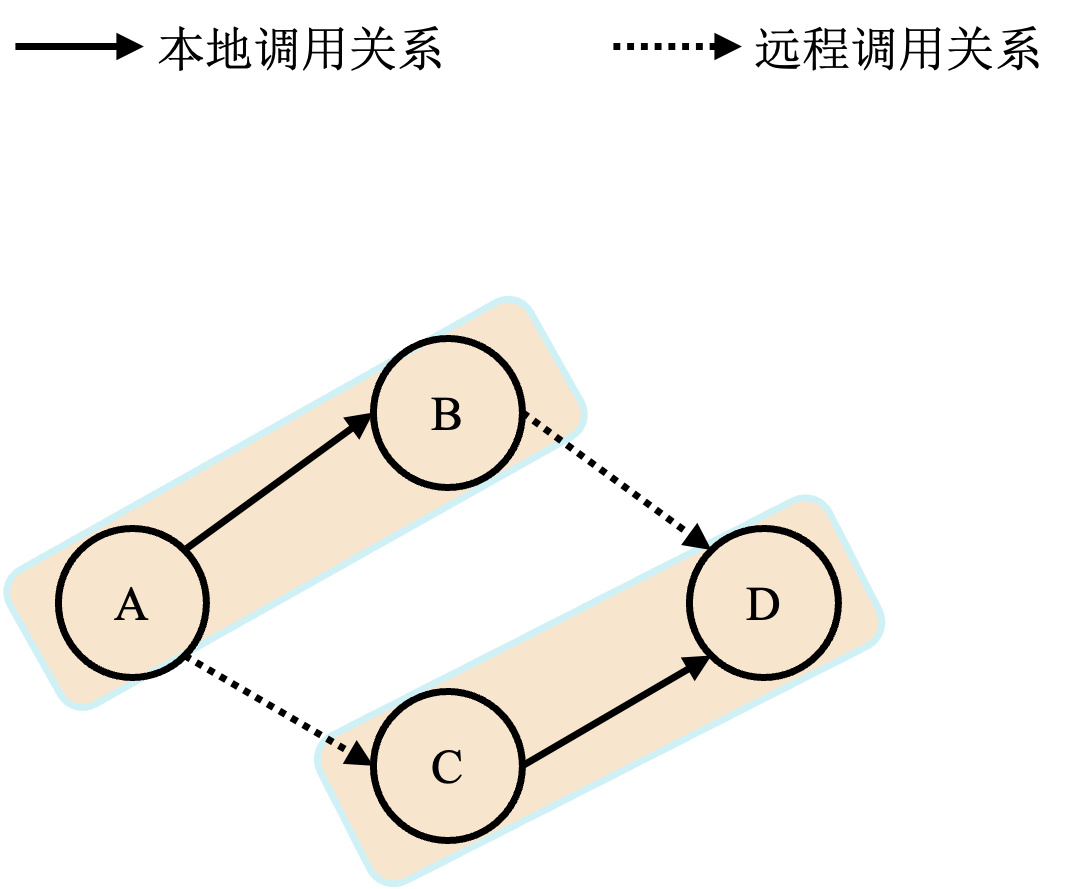
\includegraphics[width=0.48\linewidth]{figures/local.png}
    \label{fig:dismod:b}
}
\caption{分布式模块构造示例}
\label{fig:dismod}
\end{figure}

如算法\ref{seed_initialization}所示,算法首先基于函数调用关系,选择出DAG的初始节点作为分布式模块的种子,将具有较高入度的节点标记为$f_0^h$进行初始化。这些高入度节点通常代表系统中的关键组件或服务入口,通过它们作为种子可以更有效地构建围绕核心功能的分布式模块结构。初始化过程还会考虑原子函数需要的计算资源,优先选择那些被频繁调用但计算负载适中的函数作为种子节点。

\begin{algorithm}[ht]
	\caption{种子模块初始化}
	\label{seed_initialization}
	\SetAlgoLined
	\KwIn{函数调用DAG($G=(V,E)$), 原子函数集合($F$)}
	\KwOut{初始模块集合($M$), 模块数量($k$), 未分配函数集($F_{unassigned}$)}
	
	$M \gets \emptyset$; $k \gets 0$\;
	$F_{unassigned} \gets F$\;
	计算每个节点的入度和计算资源需求\;
	$H \gets \{f \in F | \text{入度}(f) < \text{阈值} \wedge Exec(f) < \text{阈值}\}$\;
	\ForEach{$f \in H$}{
		$k \gets k + 1$\;
		创建新模块 $m_k \gets \{f\}$\;
		$M \gets M \cup \{m_k\}$\;
		$F_{unassigned} \gets F_{unassigned} \setminus \{f\}$\;
	}
	\Return{$M, k, F_{unassigned}$}\;
\end{algorithm}

% \begin{algorithm}[ht]
% 	\caption{自适应分布式化算法}
% 	\label{grouping_algorithm}
% 	\SetAlgoLined
% 	\DontPrintSemicolon
% 	\KwIn{函数调用DAG($G$), 原子函数集合($F$), 模块数量上限($k_{max}$), 内存上限($\text{MEMLIMIT}$)}
% 	\KwOut{分布式模块集合$M = \{m_1, m_2, \ldots, m_k\}$}
	
% 	$M, k, F_{unassigned} \gets$ 种子模块初始化($G, F$)\;
% 	$M, k \gets$ 函数贪心分配($G, F_{unassigned}, M, k, k_{max}, \text{MEMLIMIT}$)\;
% 	$M, k \gets$ 模块通信优化($G, M, k, \text{MEMLIMIT}$)\;
% 	\Return{$M$}\;
% \end{algorithm}


在初始化完成后,算法采用迭代式贪心策略进行函数分配。如算法\ref{greedy_assignment}所示,具体而言,算法对当前节点按照DAG进行深度优先遍历,对于每个未分配的原子函数$f$,通过评估将其分配到现有模块$m$的成本$Cost(f,m)$,并基于一定阈值决定是否分配到该模块或创建新模块。这种贪心策略在每一步都选择局部最优解,虽然不能保证全局最优,但在实际应用中表现良好且计算效率高。

\begin{algorithm}[htbp]
	\caption{分布式模块构造:函数贪心分配}
	\label{greedy_assignment}
	\SetAlgoLined
	\DontPrintSemicolon
	\KwIn{函数调用DAG($G$), 未分配函数集($F_{unassigned}$), 模块集合($M$), 当前模块数($k$), 模块数上限($k_{max}$), 内存上限($\text{MEMLIMIT}$)}
	\KwOut{更新后的模块集合($M$), 更新后的模块数量($k$)}
	
	\While{$F_{unassigned} \neq \emptyset$}{
		按深度优先遍历顺序选择函数 $f \in F_{unassigned}$\;
		$best\_cost \gets \infty$; $best\_module \gets$ NULL\;
		\ForEach{$m \in M$}{
			计算分配成本 $cost \gets \frac{Exec(f)}{Cap(m) \cdot \sum_{g \in m} (Freq(f, g) + Freq(g,f))}$\;
			\If{$cost < best\_cost$ \textbf{and} $Memory(m \cup \{f\}) \leq \text{MEMLIMIT}$}{
				$best\_cost \gets cost$\;
				$best\_module \gets m$\;
			}
		}
		\eIf{$best\_module \neq$ NULL}{
			$best\_module \gets best\_module \cup \{f\}$ \tcp*{分配函数到最优模块}
		}{
			\If{$k < k_{max}$}{
				$k \gets k + 1$\;
				创建新模块 $m_k \gets \{f\}$\;
				$M \gets M \cup \{m_k\}$\;
			}\Else{
				$m_{min} \gets \arg\min_{m \in M} Memory(m)$\;
				$m_{min} \gets m_{min} \cup \{f\}$ \tcp*{分配到内存占用最小的模块}
			}
		}
		$F_{unassigned} \gets F_{unassigned} \setminus \{f\}$\;
	}
	\Return{$M, k$}\;
\end{algorithm}

原子函数的分配成本由两部分组成:函数执行开销(包括执行时间和内存占用)以及函数间的调用频率。这两个因素直接影响了系统的响应时间和资源利用率。成本函数定义如下:

\begin{equation}
	Cost(f, m) = \frac{Exec(f)}{Cap(m) \cdot \sum_{g \in m} (Freq(f, g) + Freq(g,f))}
\end{equation}

\noindent 式中:$Exec(f)$表示原子函数$f$的执行开销,执行时间和内存使用的积;$Cap(m)$表示节点对模块$m$的计算能力,反映了模块所在节点的处理能力,通过对于节点的CPU性能和可用内存数量计算得到;$Freq(f, g)$表示原子函数$f$调用原子函数$g$的频率,这一数据通过静态分析结合运行时采样获得。算法会按照$Cost$升序分配,Cost函数值越小,函数$f$将被分配到模块$m$中。

在分布式模块的内存和CPU资源管理中,本文定义了:

\begin{equation}
\label{eq:memory}
	Memory(m) = \sum_{f \in m} \alpha_f^m \cdot Memory(f)
\end{equation}

\noindent 式中:$Memory(m)$表示分布式模块$m$的总内存占用;$Memory(f)$表示原子函数$f$的内存需求;$\alpha$表示该原子函数在模块中的并发实例数量。并发实例数量直接影响模块的内存需求,特别是在高负载情况下,系统需要创建多个原子函数实例以处理并行请求。这种内存消耗模型使算法能够精确估计不同分配策略下的资源占用,从而避免内存溢出问题。


对于每一个分布式模块会存在一个内存使用上限$\text{MEMLIMIT}$。这个上限存在的原因是每个分布式模块被抽象为可以独立部署到分布式计算节点上的独立单元,而这个单元所在的节点是有内存限制的。算法在划分模块时严格考虑这一实际硬件限制,通过动态评估每个模块的内存占用情况,避免单个模块过度集中内存密集型函数而导致部署失败。此外,内存限制还促使系统更均衡地分配原子函数,提高整体资源利用效率。在实际部署中,$\text{MEMLIMIT}$的值可以根据目标环境动态调整,从而适应从边缘设备到云数据中心的不同规模集群环境。如果当前的分配方案导致某个模块的内存使用超过$\text{MEMLIMIT}$,算法会创建新的模块。


在基本分配完成后,算法进一步优化模块间的通信结构。如算法\ref{communication_optimization}所示,这一阶段首先计算模块间通信矩阵$C$,其中$C_{ij}$表示模块$i$与模块$j$之间的通信量,通过函数调用频率和数据传输量综合评估。基于这一矩阵,对于通信频繁且通信成本超过阈值$\theta$的模块对$(i,j)$,算法会选择性地执行以下操作之一:(1)合并模块,将两个高度相关的模块合并为一个;(2)重新分配原子函数,将模块间频繁调用的函数重新分配以减少跨模块调用;(3)建立函数并行调用制,在两个模块中保留关键函数的副本以减少远程调用。同时,算法维持一个负载均衡约束,确保合并和重分配操作不会导致任一模块的计算负载超过预设阈值$\text{MEMELIMIT}$,避免产生新的性能瓶颈。

\begin{algorithm}[htbp]
	\caption{分布式模块构造:模块通信优化}
	\label{communication_optimization}
	\SetAlgoLined
	\DontPrintSemicolon
	\KwIn{函数调用DAG($G$), 模块集合($M$), 模块数量($k$), 内存上限($\text{MEMLIMIT}$)}
	\KwOut{优化后的模块集合($M$), 更新后的模块数量($k$)}
	
	计算模块间通信矩阵 $C$,其中 $C_{ij}$ 表示模块 $i$ 与 $j$ 之间的通信量\;
	\ForEach{$(i,j)$ where $C_{ij} > \theta$}{
		\eIf{$Memory(m_i \cup m_j) \leq \text{MEMLIMIT}$}{
			$m_i \gets m_i \cup m_j$ \tcp*{合并高通信模块}
			$M \gets M \setminus \{m_j\}$\;
			$k \gets k - 1$\;
		}{
			模块间频繁调用的原子函数集合 $B_{ij} = \{f \in m_i \cup m_j | f的\text{跨模块调用频率} > \tau\}$\;
			\ForEach{$f \in B_{ij}$}{
				$RemoteCost(f) = Freq(f) \times (LatencyNetwork + SerializationTime)$\;
				$LocalCost(f) = Mem(f) \times ReplicationFactor$\;
				\eIf{$RemoteCost(f) > LocalCost(f)$}{
						\eIf{$f \in m_i$ \textbf{and} $Memory(m_j \cup \{f\}) \leq \text{MEMLIMIT}$}{
								在$m_j$中创建$f$的副本\;
						}{
								\If{$f \in m_j$ \textbf{and} $Memory(m_i \cup \{f\}) \leq \text{MEMLIMIT}$}{
										在$m_i$中创建$f$的副本\;
								}
						}
				}{
						重分配$f$到调用频率更高的模块\;
				}
			}
		}
	}
	\Return{$M, k$}\;
\end{algorithm}


对于分布式模块内部的计算优化,本算法的核心优势在于其自适应特性。算法具备多层次的自动扩展能力:在粗粒度上,可以根据可用资源动态调整分布式模块的并发数量$k$,无需重新设计分布式架构;在细粒度上,单个分布式模块内部并行执行多个原子函数,实现计算负载的动态均衡分配,尤其适合处理负载波动较大的Agent任务。

最终构造的分布式模块内函数间具有较高的调用频率和依赖关系,减少了远程调用的延迟和开销。模块间通信开销最小化,减少了网络流量和序列化/反序列化开销。各模块的计算资源消耗相对均衡,避免出现计算热点和性能瓶颈。支持水平和垂直扩展,动态调整模块数量和单模块资源配置。通过冗余设计和快速故障恢复机制,确保在部分节点失效时系统仍能维持基本功能,提高了系统的整体可靠性。

\section{编译器}
\label{sec:compiler}
编译器架构如图\ref{fig:compiler}所示,主要完成以下任务:原子函数的识别、原子函数的指标统计、分布式模块的编译、针对分布式化后的程序的优化。在原子函数识别阶段,编译器会遍历程序的AST,识别出所有的原子函数。在原子函数指标统计阶段,编译器会统计每个原子函数的CPU时间消耗、内存占用、函数依赖等信息。在分布式模块编译阶段,编译器会将单机程序编译成分布式模块并对可能的并行策略做出优化。

\begin{figure}[ht]
    \centering
    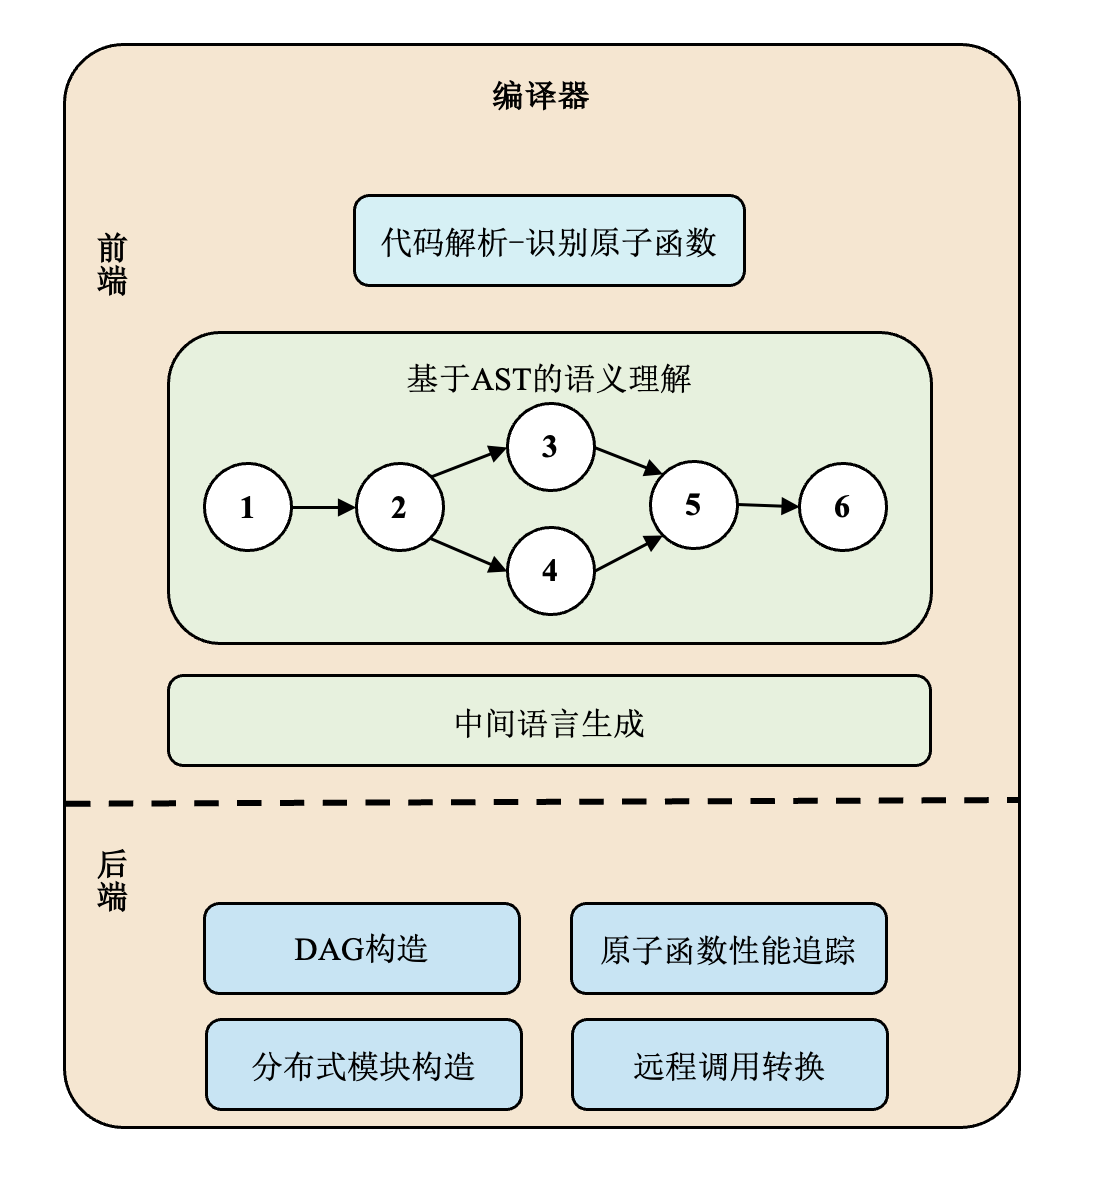
\includegraphics[width=0.55\textwidth]{compiler.png}
    \caption{编译器架构}
    \label{fig:compiler}
\end{figure}


识别原子函数。在自适应分布式框架中,编译器首先需要识别出程序中的原子函数。原子函数是指可以被执行的最小计算单元,是分布式化的基础单位。编译器通过以下步骤完成原子函数的识别:

编译器首先将源代码解析为AST,提取代码的结构信息。函数单元划分:通过遍历AST,识别出所有的函数定义。根据函数的调用深度,判断其是否适合作为原子函数。对识别出的原子函数进行标记,为后续的分布式化做准备。

构建DAG。首先,编译器通过静态调用分析,遍历整个AST,识别每个函数直接调用的其他函数,建立函数间的直接调用关系图。同时,控制流分析用于分析条件分支和循环结构,识别可能的执行路径,进一步完善函数间的依赖关系。

在构建过程中,以函数为节点,以调用关系为有向边,边的权重表示调用频率。同时,根据函数调用频率计算边的权重。

通过构建精确的函数依赖DAG,编译器能够全面理解程序的结构特性,为后续的分布式转换提供详细的依据,从而实现高效的任务分解、调度和优化,最终实现自适应的分布式执行。

统计指标。编译器需要对每个原子函数进行性能指标的统计,这些指标将作为后续任务调度和资源分配的重要依据:

通过插桩技术和采样分析,记录函数的执行时间,评估其计算复杂度和处理能力需求。统计函数在执行过程中的内存分配和释放情况,评估其内存资源需求。

分布式模块构造。编译器基于前述原子函数划分与性能指标,实施系统性转换构建分布式模块:首先构建分布式模块注册表,记录所有模块的依赖关系和性能特征;然后为原子函数参数和返回值自动生成类型安全的序列化/反序列化代码,支持各类复杂数据结构的网络传输;生成高效RPC接口,内置错误处理、重试逻辑和负载均衡策略。这种多层架构设计实现了单体应用到分布式系统的自动化转换,无需开发者手动重构代码或掌握复杂的分布式编程模型,极大地简化了分布式系统开发流程。

编译器实现了基于函数调用关系和资源特性的自动模块划分算法,无需开发者手动定义微服务边界,大幅简化了从单体应用到微服务架构的转换过程。能够自动识别并转换跨模块调用,将普通函数调用转换为网络RPC调用,同时保持代码的清晰度和可维护性。通过打桩分析的方式,系统能够提取和计算函数的性能特征(执行时间、内存使用等),为智能资源分配提供基础数据。然而,这些优化后的分布式模块需要在适当的运行环境中部署和调度才能发挥其最大效能。因此,下一节将介绍框架的服务器组件,探讨如何构建高效的分布式执行环境,实现分布式模块的动态部署、资源管理机制。

\section{服务器}
\label{sec:server}

服务器架构如图\ref{fig:server}所示,是自适应分布式化框架的中央协调组件,负责分布式模块的部署、管理与资源调度。与传统的服务器不同,本框架的服务器组件专门设计用于处理由编译器生成的分布式模块,提供自动化的生命周期管理和智能资源分配,构建了一个对上层应用透明的分布式执行环境。

\begin{figure}[ht]
    \centering
    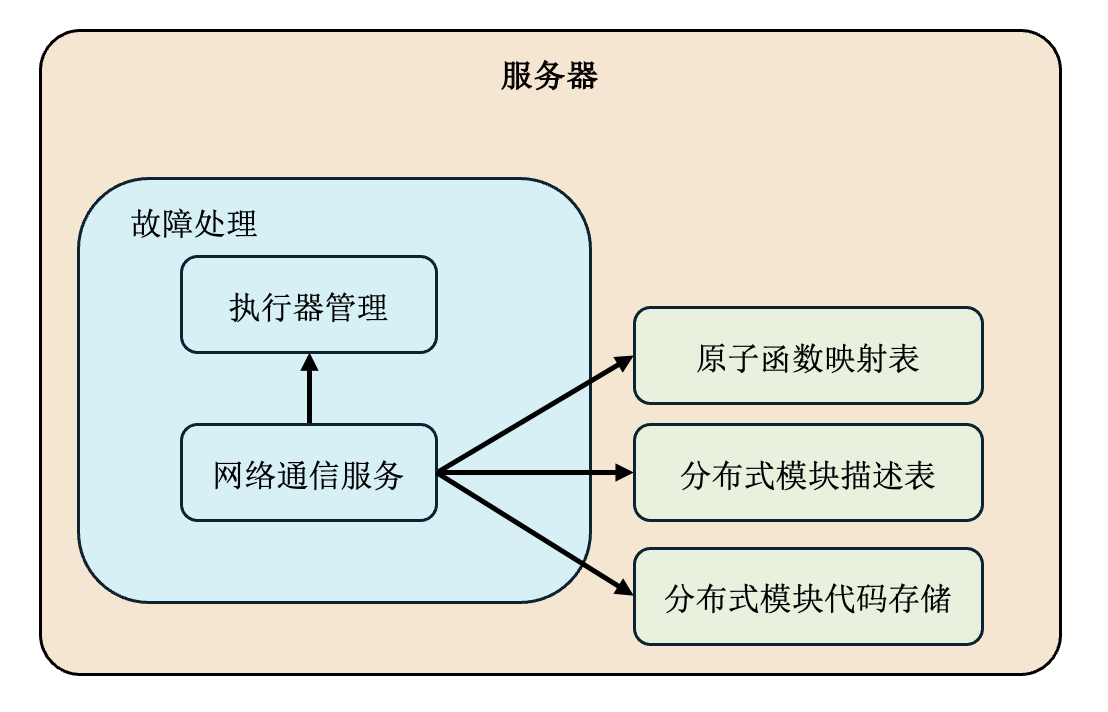
\includegraphics[width=0.6\textwidth]{server.png}
    \caption{服务器架构}
    \label{fig:server}
\end{figure}

服务器的核心设计原则是采用轻量级控制平面设计,将大部分计算密集型任务委托给执行器\ref{sec:executor},自身专注于元数据管理和调度决策,避免成为系统性能瓶颈。服务器维护全局资源视图和分布式模块映射关系,为智能调度提供决策依据。

服务器组件由三个心模块构成,分别是元数据管理模块、部署管理模块和路由引擎模块。

元数据管理维护两类关键元数据:分布式模块描述表和原子函数映射表。前者包含模块标识、资源需求、依赖关系和状态信息,由编译器生成并在部署时注册。后者记录原子函数与分布式模块的对应关系,支持O(1)复杂度的快速查询,确保调用请求能准确定位目标执行器。

函数映射采用双层哈希表实现,确保在大规模分布式环境中保持高效的查询性能。服务器在启动时加载分布式模块配置,构建内存索引,并周期性持久化以支持故障恢复。

部署管理模块实现了自动化的部署流程,将编译器生成的分布式模块转换为可执行实体。资源管理采用弹性扩缩容策略,根据实时负载动态调整执行器实例数量,同时考虑资源利用率和请求延迟等多维度指标,在性能和成本之间寻求平衡。

路由引擎模块作为调用网关,实现了透明的函数调用路由机制。首先接收客户端函数调用请求,解析目标函数标识和参数数据其次查询函数映射表,确定目标函数所属的分布式模块和执行器实例然后检查执行器健康状态,必要时触发故障转移或重新部署然后转发调用请求至目标执行器,同时收集性能遥测数据最后等待执行结果并返回给客户端,处理潜在的超时和错误情况

路由层实现了多种优化技术,包括结果缓存、连接池复用和请求批处理,有效减少了网络开销和延迟,提高了系统吞吐量。

此外,服务器采用轻量级的基于HTTP的RPC协议,支持JSON和cloudpickle两种序列化格式。JSON格式适用于简单数据类型,具有良好的可读性和兼容性。二进制格式(cloudpickle)支持复杂Python对象的高效序列化,适用于大数据量传输

协议实现了自适应压缩和传输优化,能根据数据特征自动选择最优传输策略,平衡网络开销与CPU消耗。

服务器还实现了多层次的故障检测与恢复机制。定期探测执行器状态,通过心跳机制快速识别故障节点。检测到执行器异常时,自动触发重启流程,恢复服务可用性。利用持久化的元数据,在执行器重启后恢复运行状态。j对失败的函数调用实施指数退避策略的自动重试机制。

故障恢复策略考虑了分布式模块的依赖关系,确保按正确顺序重启相关服务,最小化故障影响范围。

服务器与编译器\ref{sec:compiler}和执行器\ref{sec:executor}紧密协作,共同构建了一个自适应的分布式执行框架。编译器负责静态分析和模块划分,服务器管理部署和调度,执行器实现实际计算,这种分层设计既保持了系统的高内聚低耦合特性,又提供了面向不同场景的优化空间。

\section{执行器}
\label{sec:executor}
执行器架构如图\ref{fig:executor}所示,作为框架的核心组件,负责加载和执行分布式模块中的函数。执行器提供了轻量级的函数执行环境,支持同步和异步函数的调用,具有高效、灵活的特点,为分布式应用提供了强大的计算支持。

\begin{figure}[ht]
    \centering
    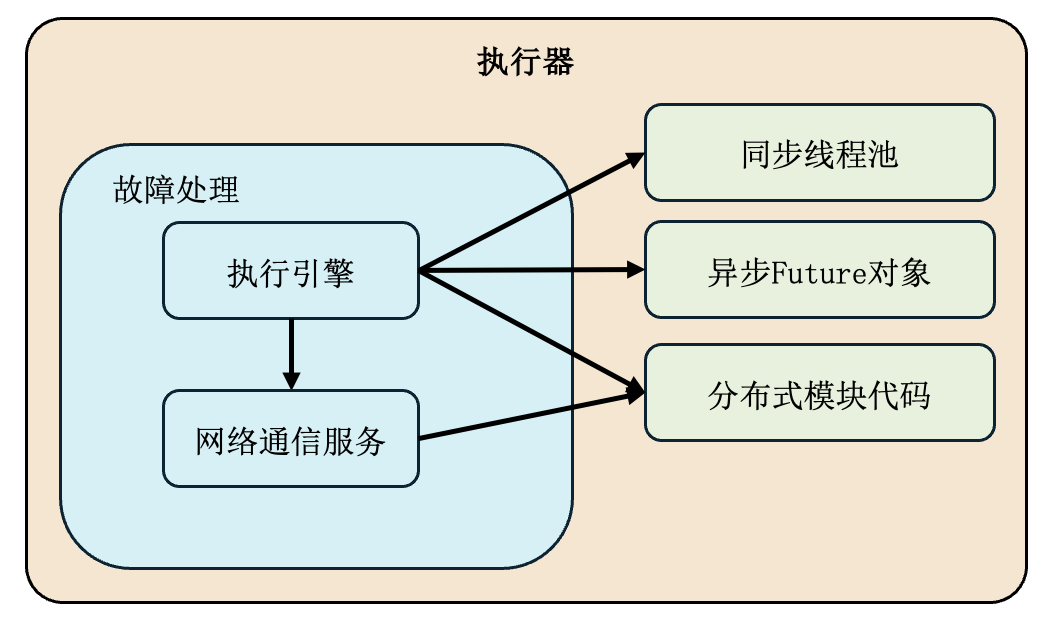
\includegraphics[width=0.6\textwidth]{executor.png}
    \caption{执行器架构}
    \label{fig:executor}
\end{figure}

当执行器启动时,它会从服务器加载特定分布式模块及其配置文件。为减少代码传输的开销,每个执行器都持有完整的代码片段副本。执行器准备就绪后,将负责管理当前分布式模块中逻辑分配的原子函数的调用和执行。对于远程调用,执行器会检查目标原子函数是否在同一分布式模块中:如果是,则可以在本地直接调用该原子函数;否则,执行器将尝试从管理器获取并缓存拥有目标原子函数的分布式模块的端点信息,然后生成RPC请求。

执行器采用无状态且轻量级设计,具有极小的资源占用特点。它们与自动伸缩和基于重试的容错机制高度兼容,能够快速扩展或切换内部分布式模块,特别适合于Serverless基础设施。这种设计理念使执行器能够根据工作负载动态调整资源分配,在保持高性能的同时确保系统的弹性和可靠性。执行器主要由以下三个核心组件构成:初始化组件、执行引擎和API服务层。

初始化组件实现了动态模块加载机制,通过以下步骤完成模块加载和函数注册。首先,读取模块配置文件,解析函数元数据;然后,编译并执行源代码文件,捕获全局命名空间;最后,从命名空间中查找并注册目标函数。这种动态加载方式避免了硬编码依赖,提高了系统的灵活性和可扩展性。

执行对同步函数通过线程池执行,避免阻塞主事件循环;异步函数直接在事件循环中执行,充分利用异步IO能力。执行器会自动检测函数类型,选择合适的执行策略,并处理各种异常情况,包括函数不存在、参数无效和执行错误等。

API服务层基于aiohttp框架实现,提供了RESTful API接口,支持函数调用,支持JSON和cloudpickle序列化方式、模块信息查询和健康状态检查。实现了完善的错误处理机制,包括参数验证和类型检查、异常捕获和日志记录、标准化的错误响应。

执行器作为分布式系统的核心执行组件,通过其高效的函数加载与执行机制、灵活的序列化支持和强大的并发处理能力,为分布式应用提供了可靠、高效的函数执行环境。其设计理念和技术实现为构建大规模分布式计算系统提供了有力支持。

\section{本章小结}

本文提出了一种创新的自适应分布式化框架,该框架能够自动将单机程序转换为分布式应用,通过多层次抽象、资源感知的智能分组、编译时静态优化与运行时动态调度相结合、轻量级执行环境以及透明的分布式调用等核心特性,实现了程序的无感知分布式化。框架首先通过设定合理的函数深度参数$h$,在保持程序语义不变的前提下为分布式化提供理想粒度,将程序拆分为多个原子函数;随后利用基于抽象语法树的静态分析方法构建原子函数调用DAG,并通过轻量级插桩技术精确统计每个原子函数的CPU时间消耗、内存占用和调用频率等关键指标;在此基础上,框架采用三阶段的分组聚类算法(初始化、迭代优化和通信优化)将原子函数智能分组为分布式模块,该算法综合考虑了计算密集型和内存密集型函数的特点,在最小化模块间通信开销的同时确保系统资源均衡分配;框架的服务器组件实现了分布式模块的动态部署、资源管理和故障恢复,提供了高可用的分布式运行环境;执行器采用无状态设计,具有极小的资源占用特点,支持同步和异步函数的高效调用,特别适合于Serverless环境;此外,框架还实现了透明的函数调用路由机制,自动将跨模块的函数调用转换为网络RPC调用,通过优化的序列化和通信协议最小化了分布式调用的开销。这一自适应分布式化框架显著简化了从单体应用到分布式系统的转换过程,无需开发者手动定义微服务边界或编写分布式协调代码,使得普通应用能够无感知地享受分布式计算带来的扩展性和性能提升。